\begin{figure}[ht] %s state preferences regarding figure placement here

% use to correct figure counter if necessary
%\renewcommand{\thefigure}{2}

\centering
\subfigure[URL reference]{%
\label{fig:verification-a}%
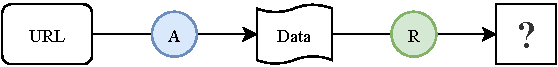
\includegraphics[scale=0.74]{figures/fig4a.pdf}} \\
\subfigure[Content URI reference]{%
\label{fig:verification-b}%
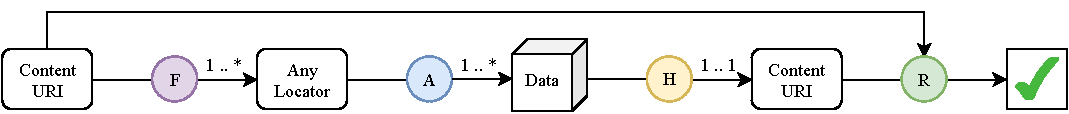
\includegraphics[scale=0.74]{figures/fig4b.pdf}} \\
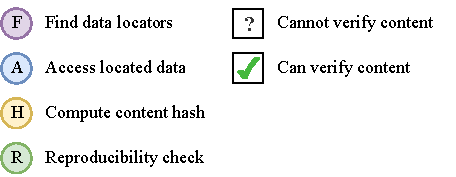
\includegraphics[scale=.9]{figures/fig4legend.pdf}%

\caption{Content resolution and verification for references that use location- versus content-based identifiers. \subref{fig:verification-a} Location-based identifiers (e.g. URLs) cannot verify the authenticity of retrieved content. \subref{fig:verification-b} Content-based identifiers (e.g. Content URIs) can verify the authenticity of retrieved data by comparing the hash of the retrieved data with the hash embedded in the identifier.
}%

\label{fig:verification} % \label works only AFTER \caption within figure environment

\end{figure}
